\documentclass[a4paper]{article}
\usepackage{amsmath,amsthm,enumitem}
\usepackage[margin=3cm]{geometry}
\usepackage[T1]{fontenc}
\usepackage[bitstream-charter,cal]{mathdesign}
\linespread{1.15}
\usepackage{luatexja}
\theoremstyle{definition}
\newtheorem{prb}{}
\renewcommand{\theprb}{問\arabic{prb}}

\usepackage{tikz}
\usetikzlibrary{calc,decorations.markings}

\renewcommand{\Re}{\operatorname{Re}}
\renewcommand{\Im}{\operatorname{Im}}
\renewcommand{\H}{\mathbb{H}}
\newcommand{\C}{\mathbb{C}}
\newcommand{\R}{\mathbb{R}}
\newcommand{\Z}{\mathbb{Z}}
\newcommand{\e}{\varepsilon}
\newcommand{\f}{\varphi}
\newcommand{\PSL}{\operatorname{PSL}}
\renewcommand{\tilde}{\widetilde}
\renewcommand{\bar}{\overline}

\begin{document}

\title{複素解析学I演習2023年}
\date{}
\maketitle


\begin{prb}[フックス群としてのモジュラー群]
複素数体$\C$の部分集合$A$に対して、成分$a,b,c,d$が$A$の元で$ad-bc=1$を満たす一次分数変換$f(z)=(az+b)/(cz+d)$の集合を$\PSL(2,A)$と書く.
特に$\PSL(2,\Z)$を\emph{モジュラー群}と呼ぶ.
上半平面$\H:=\{z\in\C:\Im z>0\}$の部分集合$D:=\{z\in\H:|z|>1,\ |\Re z|<\frac12\}$を定義する.
\begin{enumerate}[label=(\arabic*)]
\item $\PSL(2,\R)$の元$f$は全単射写像$\H\to\H$を定義することを示せ.
\item $\PSL(2,\Z)$は$S(z):=-1/z$と$T(z):=z+1$によって生成されることを示せ.つまり、全ての元が$S^{\pm1}$と$T^{\pm1}$の有限回の合成として表れることを示せ.
\item 集合$D$は$\PSL(2,\Z)$の\emph{基本領域}であることを示せ.つまり、次の二つが成り立つことを示せ:
\begin{enumerate}[label=(\alph*)]
\item 任意の点$z\in\H$に対して$f(z)\in\bar D$を満たす$f\in\PSL(2,\Z)$が少なくとも一つ存在する.
\item 任意の点$z\in\H$に対して$f(z)\in D$を満たす$f\in\PSL(2,\Z)$が多くとも一つ存在する.
\end{enumerate}
\item $\PSL(2,\Z)$は$\H$に\emph{真性不連続に作用}することを示せ.つまり、任意の点$z\in\H$に対して軌道$\{f(z):f\in\PSL(2,\Z)\}$が離散集合であることを示せ.
\end{enumerate}
\end{prb}


\begin{prb}[カラテオドリ級関数集合の極点]
開単位円板上で定義された正則関数$f$が$f(0)=1$を満たすとする.
もし任意の$|z|<1$を満たす複素数$z$に対して$\Re f(z)>0$ならば、$f$を\emph{カラテオドリ級}の関数という.
関数$f$が冪級数展開$f(z)=1+2\sum_{k=1}^\infty c_kz^k$を持つとする.
\begin{enumerate}[label=(\arabic*)]
\item 正の整数$k$と実数$0<r<1$に対して次の式を示せ:
\[c_kr^k=\frac1{2\pi}\int_0^{2\pi}\Re f(re^{i\theta})e^{-ik\theta}\,d\theta.\]
\item 次の二つの条件が同値であることを示せ:
\begin{enumerate}[label=(\alph*)]
\item 関数$f$がカラテオドリ級である.
\item 任意の正の整数$n$に対して点$(c_1,\cdots,c_n)\in\C^n$は$\theta\in[0,2\pi)$によって媒介変数表示された曲線$(e^{-i\theta},\cdots,e^{-in\theta})\in\C^n$の凸包絡の元である.
\end{enumerate}
\end{enumerate}
\end{prb}


\begin{prb}[アールフォルス・清水標数]
複素平面上の有理型関数$f$を考える.
次のように$r\ge0$に対する関数$A(\cdot,f)$を定義する:
\[A(r,f):=\frac1\pi\int_{\sqrt{x^2+y^2}\le r}f^\#(x+iy)^2\,dx\,dy,\qquad\text{ただし、}\ f^\#(z):=\frac{|f'(z)|}{1+|f(z)|^2},\quad z\in\C.\]
関数$f^\#$を$f$の\emph{球面導関数}と呼ぶ.
\begin{enumerate}[label=(\arabic*)]
\item 任意の点$(x,y)\in\R^2$に対して、
\[\frac1\pi\,f^\#(x+iy)^2=\frac{\partial Q}{\partial x}(x,y)-\frac{\partial P}{\partial y}(x,y)\]
を満たす実平面$\R^2$上の実関数$P$と$Q$を求め、関数$K(x,y):=1+|f(x+iy)|^2$を用いて表せ.
\item グリーンの定理と偏角の原理を用いて$r\ge0$に対して次の式が成り立つことを示せ:
\[\int_0^rA(t,f)\frac{dt}t=\int_0^rn(t,f)\frac{dt}t+\frac1{2\pi}\int_0^{2\pi}\log\sqrt{1+|f(re^{i\theta})|^2}\,d\theta-\log\sqrt{1+|f(0)|^2}.\]
ただし、$n(r,f)$は閉円板$\bar{B(0,r)}$内にある重複度を込めて数えた$f$の極の数である.
左辺の関数を$f$の\emph{アールフォルス・清水標数}と呼ぶ.
\item 球面導関数$f^\#$が有界ならば、ある定数$C>0$が存在して、全ての$z\in\C$に対して$|f(z)|\le Ce^{|z|^2}$であることを示せ.特に、$f$は$\C$全体上正則である.
\end{enumerate}
\end{prb}

\begin{prb}[四分円上のディリクレ問題]
領域$\Omega:=\{(x,y)\in\R^2:x^2+y^2<1,\ x>0,\ y>0\}$上に定義された調和関数$v\in C^2(\Omega,\R)$が次の境界値条件を満たすとする:
各点$(x_0,y_0)\in\partial\Omega$に対して
\[\lim_{(x,y)\to(x_0,y_0)}v(x,y)=\begin{cases}
1&\text{ if }y_0>0,\\
0&\text{ if }y_0=0\text{ and }0<x_0<1.
\end{cases}\]
\begin{enumerate}[label=(\arabic*)]
\item 反射原理を用いて$v$は領域$\tilde\Omega:=\{(x,y)\in\R^2:x^2+y^2<1,\ x>0\}$上の調和関数$\tilde v\in C^2(\tilde\Omega,\R)$に拡張されることを示せ.
\item 適切な等角変換とポアソン積分を用いて$v$を求めよ.
\end{enumerate}
\end{prb}


\newpage

\begin{proof}[Solution of 1]
(1)
Let $f(z)=(az+b)/(cz+d)$ with $a,b,c,d\in\R$ such that $ad-bd=1$.
Since it has the inverse transform $z\mapsto(dz-b)/(-cz+a)$ that is also an element of $\PSL(2,\R)$, it is enough to show the well-definedness $f(z)\in\H$ for $z\in\H$.
Let $z=x+iy\in\H$ with $y>0$.
Then,
\[\Im f(z)=\Im\frac{ax+b+iay}{cx+d+icy}=\frac{ay(cx+d)-(ax+b)cy}{(cx+d)^2+(cy)^2}\frac y{(cx+d)^2+(cy)^2}>0,\]
so $f(z)\in\H$.

(2)
Let $f(z)=(az+b)/(cz+d)$ with $a,b,c,d\in\Z$ such that $ad-bd=1$.
Consider the following two kinds of moves of $f$:
\begin{itemize}
\item When $|a|<|c|$, we take
\[Sf(z)=\frac{-cz-d}{az+b}.\]
\item When $|a|\ge|c|>0$, with $q,r\in\Z$ such that $a=qc+r$ and $0\le r<|c|$, we take
\[T^{-q}f(z)=\frac{rz+b-qd}{cz+d}.\]
\end{itemize}
By repeating the two moves alternately, we arrive at $c=0$ in finitely many steps because $|c|$ strictly decreases.
Then, since $ad-bc=1$, we may assume $a=d=1$ so that $(az+b)/(cz+d)=z+b=T^b(z)$.


(3)
(a)
Let $z_0\in\H$.
We may assume $\Re z_0\in[-\frac12,\frac12)$ by taking $T^q$ on $z_0$ for appropriate $q\in\Z$.
Define a sequence $z_n\in\H$ inductively by
\[z_n:=T^{-\lfloor\Re S(z_{n-1})+\frac12\rfloor}S(z_{n-1}),\qquad n\ge1.\]
Then, one can show $\Re z_n\in[-\frac12,\frac12)$ for all $n$.
Since
\[\Im z_n=\Im S(z_{n-1})=\frac{\Im z_{n-1}}{(\Re z_{n-1})^2+(\Im z_{n-1})^2}\ge g(\Im z_{n-1}),\]
where $g(y):=4y/(1+4y^2)$, and since $g^n(y)\uparrow\frac{\sqrt3}2$ for $0<y<\frac{\sqrt3}2$ as $n\to\infty$, there is $n$ such that
\[-\frac12\le\Re z_n<\frac12,\qquad\Im z_n>\frac{\sqrt3}4.\]
If $|z_n|\ge1$, then we are done, so assume $|z_n|<1$.
Now we have three possibilities: $|z_n-1|<1$, $|z_n+1|<1$, or $\min\{|z_n-1|,|z_n+1|\}\ge1$.
For each case, we can check that $T^{-1}Sz_n$, $TSz_n$, $Sz_n$ is contained in $\bar D$, respectively.

(b)
For $z\in D$, let $w=(az+b)/(cz+d)\in D$ with $a,b,c,d\in\Z$ such that $ad-bd=1$.
It suffices to show $c=0$.
Suppose $c\ne0$.
Note that $|z-n|>1$ and $|w-n|>1$ for every integer $n$ since $z,w\in D$.
Write
\[1<|w-n|=\left|\frac{az+b}{cz+d}-n\right|\le\left|\frac{az+b}{cz+d}-\frac ac\right|+\left|n-\frac ac\right|=\left|\frac1{c(cz+d)}\right|+\left|n-\frac ac\right|,\qquad n\in\Z.\]
If $|c|\ge2$, then by taking $n$ such that $|n-(a/c)|\le\frac12$, the estimate $|c(cz+d)|\ge|c|^2\Im z>2\sqrt3$ leads a contradiction to the above inequality.
If $|c|=1$, then since $a/c$ is an integer, by letting $n=a/c$, we have a contradiction $|c(cz+d)|=|z+cd|>1$ from the assumption $z\in D$.
Thus, $c=0$, and we are done.

(4)
Suppose the orbit $\{f(z):f\in\PSL(2,\Z)\}$ is not discrete.
Then, there is $z_0\in\H$ and a sequence $f_n\in\PSL(2,\Z)$ such that $f_n(z)\ne z_0$ for all $n$ and $f_n(z)\to z_0$ as $n\to\infty$.
We may assume $z,z_0\in\bar D$ by the part (a) of (3).
Note that there are only finitely many $f\in\PSL(2,\Z)$ such that $f(\bar D)\cap\bar D\ne\varnothing$.
Let $P$ be the set of such $f$.


If $z_0\in D$, then $f_n(z)$ eventually belongs to $D$, which is impossible by the part (b) of (3).
If $z_0\in$

\end{proof}

\begin{proof}[Remark]
A discrete subgroup of $\PSL(2,\R)$ and $\PSL(2,\C)$ is called a \emph{Fuchsian group} and a \emph{Kleinian group} respectively.
It is known that a subgroup of $\PSL(2,\R)$ is discrete if and only if it properly discontinuously acts on $\H$.
There is a more generalized theorem used for verifying a group generated by several elements of $\PSL(2,\R)$ is Fuchsian, the \emph{Poincare polygon theorem}.
It states that if there is a polygon in $\H$ satisfying two conditions called a side pairing condition and elliptic cycle condition is realized as a fundamental domain, so the group acts on $\H$ properly discontinuously.
\end{proof}

\newpage
\begin{proof}[Solution of 2]
(1)
Suppose $k>0$ first.
The Cauchy integral formula writes
\begin{align*}
2c_kk!=\pd[k]{f}{z}(0)=\frac{k!}{2\pi i}\int_{|z|=r}\frac{f(z)}{z^{k+1}}\,dz=\frac{k!}{2\pi}\int_0^{2\pi}\frac{f(re^{i\theta})}{(re^{i\theta})^k}\,d\theta,
\end{align*}
and it implies
\[2c_kr^k=\frac1{2\pi}\int_0^{2\pi}f(re^{i\theta})e^{-ik\theta}\,d\theta.\]
Since $f(z)\,z^k$ is analytic, the Cauchy theorem can be applied to get
\[0=\frac1{2\pi i}\int_{|z|=r}f(z)\,z^k\,dz=\frac1{2\pi}\int_0^{2\pi}f(re^{i\theta})r^ke^{ik\theta}\,d\theta,\]
and it implies
\[0=\frac1{2\pi}\int_0^{2\pi}\bar{f(re^{i\theta})}e^{-ik\theta}\,d\theta.\]
By combining the above two equations, we obtain the formula.
For $k=0$, applying the Cauchy theorem for $f$, we have
\[c_0=f(0)=\frac1{2\pi i}\int_{|z|=r}\frac{f(z)}z\,dz=\frac1{2\pi}\int_0^{2\pi}\Re f(re^{i\theta})\,d\theta.\]

Alternatively, we can show the same result using the orthogonal relation of complex exponential functions.
An easy computation shows the identity
\begin{align*}
\Re f(re^{i\theta})
&=\frac12[f(re^{i\theta})+\bar{f(re^{i\theta})}]\\
&=\frac12\left[\left(1+\sum_{k=1}^\infty2c_k(re^{i\theta})^k\right)+\bar{\left(1+\sum_{k=1}^\infty2c_k(re^{i\theta})^k\right)}\right]\\
&=\frac12\left[\left(1+\sum_{k=1}^\infty2c_kr^ke^{ik\theta}\right)+\left(1+\sum_{k=1}^\infty2\bar{c_k}r^ke^{-ik\theta}\right)\right]\\
&=\sum_{k=-\infty}^\infty c_kr^{|k|}e^{ik\theta}.
\end{align*}
From the uniform convergence of the power series on the compact set $\{z:|z|\le(r+1)/2\}$, it follows that
\[\frac1{2\pi}\int_0^{2\pi}\Re f(re^{i\theta})e^{-ik\theta}\,d\theta=\sum_{l=-\infty}^{\infty}c_lr^{|l|}\frac1{2\pi}\int_0^{2\pi}e^{il\theta}e^{-ik\theta}\,d\theta=\sum_{l=-\infty}^{\infty}c_lr^{|l|}\delta_{kl}=c_kr^{|k|}.\]

(2)
(b)$\Rightarrow$(a)
Denote by $K_n$ the convex hull of the curve $\theta\mapsto(e^{-i\theta},\cdots,e^{-in\theta})\in\C^n$.
Suppose first that $(c_1,\cdots,c_n)\in K_n$.
For each $n$, there exists a finite sequence of pairs $(\lambda_{n,j},\theta_{n,j})_j$ having the following convex combination
\[(c_1,\cdots,c_n)=\sum_j\lambda_{n,j}(e^{-i\theta_{n,j}},\cdots,e^{-in\theta_{n,j}})\]
with coefficients $\lambda_{n,j}\ge0$ such that $\sum_j\lambda_{n,j}=1$.
Define
\[f_n(z):=\sum_j\lambda_{n,j}\frac{e^{i\theta_{n,j}}+z}{e^{i\theta_{n,j}}-z},\]
which has positive real part on $|z|<1$ because $\Re(e^{i\theta_{n,j}}+z)/(e^{i\theta_{n,j}}-z)>0$ for $|z|<1$.
Then,
\begin{align*}
f_n(z)
&=\sum_j\lambda_{n,j}(1+\sum_{k=1}^\infty2e^{-ik\theta_{n,j}}z^k)=1+\sum_{k=1}^n2c_kz^k+\sum_{k=n+1}^\infty\left(\sum_j2\lambda_{n,j}e^{-ik\theta_{n,j}}\right)z^k
\end{align*}
implies
\begin{align*}
|f_n(z)-f(z)|
&=\left|\sum_{k=n+1}^\infty\left(\sum_j2\lambda_{n,j}e^{-ik\theta_{n,j}}\right)z^k-\sum_{k=n+1}^\infty2c_kz^k\right|\\
&\le\sum_{k=n+1}^\infty\left|\left(\sum_j2\lambda_{n,j}e^{-ik\theta_{n,j}}\right)-2c_k\right||z|^k\le\sum_{k=n+1}^\infty4|z|^k
\end{align*}
converges to zero for $|z|<1$.
Therefore, $f$ has a non-negative real part on the open unit disk.
The non-negativity can be strengthened to positivity by the open mapping theorem, so $f$ belongs to the Carath\'eodory class.

(a)$\Rightarrow$(b)
Conversely, suppose that $f$ is in the Carath\'eodory class.
Let $(\gamma_1,\cdots,\gamma_n)$ be any point on the surface $\partial K_n$ of $K_n$ and $S$ any supporting hyperplane of $K_n$ tangent at $(\gamma_1,\cdots,\gamma_n)$.
Let $(u_1,\cdots,u_n)\in\C^n$ be the outward unit normal vector of the supporting hyperplane $S$.
Note that this outward unit normal vector is uniquely determined for each hyperplane $S$ with respect to the real inner product structure on the $2n$-dimensional real vector space $\C^n$ given by
\[\langle(z_1,\cdots,z_n),(w_1,\cdots,w_n)\rangle=\sum_{k=1}^n(\Re z_k\Re w_k+\Im z_k\Im w_k)=\Re\sum_{k=1}^nz_k\bar w_k.\]
Then, we know that $\sum_{k=1}^n|u_k|^2=1$ and the maximum
\[M:=\max_{(x_1,\cdots,x_n)\in K_n}\ \Re\sum_{k=1}^nx_k\bar u_k>0\]
is attained at $(\gamma_1,\cdots,\gamma_n)$.
Our goal is now to verify the bound
\[\Re\sum_{k=1}^nc_k\bar u_k\le M\]
from the assumption that $f$ is of Carath\'eodory class.
Once the bound is obtained, then it means that $(c_1,\cdots,c_n)$ is contained in the same side as $K_n$ of arbitrary hyperplanes tangent to $K_n$, so we finally conclude $(c_1,\cdots,c_n)\in K_n$.

Since for any $\theta\in[0,2\pi)$ the point $(e^{-i\theta},\cdots,e^{-in\theta})$ is in $K_n$, we have
\[\Re\sum_{k=1}^ne^{-ik\theta}\bar u_k\le M.\]
For $\e>0$, we have
\[\Re\sum_{k=1}^n\frac1{r^k}e^{-ik\theta}\bar u_k\le M+\e\]
for any $0<r<1$ sufficiently close to $1$, thus we can write
\begin{align*}
\Re\sum_{k=1}^nc_k\bar u_k
&=\Re\sum_{k=1}^n\frac1{2\pi r^k}\int_0^{2\pi}\Re f(re^{i\theta})e^{-ik\theta}\bar u_k\,d\theta\\
&=\frac1{2\pi}\int_0^{2\pi}\Re f(re^{i\theta})\Re\sum_{k=1}^n\frac1{r^k}e^{-ik\theta}\bar u_k\,d\theta\\
&\le\frac1{2\pi}\int_0^{2\pi}\Re f(re^{i\theta})\,d\theta\cdot(M+\e)\\
&=\Re f(0)(M+\e)=M+\e
\end{align*}
thanks to the part (1) and the positivity of $\Re f$, and by limiting $r\to1$ from left we get the bound we want.
\end{proof}


\newpage
\begin{proof}[Solution of 3]
(1)
\[\frac{du\wedge dv}{\pi(1+u^2+v^2)^2}=d\left(-\frac v{2\pi(1+u^2+v^2)}\,du+\frac u{2\pi(1+u^2+v^2)}\,dv\right)\]


\[P=-\frac{K_y}{4\pi K},\qquad Q=\frac{K_x}{4\pi K}.\]

(2)
Since the equation holds for $r=0$, it suffices to show the differentiated equation
\[A(r,f)=n(r,f)+\frac r{2\pi}\frac d{dr}\int_0^{2\pi}\log\sqrt{1+|f(re^{i\theta})|^2}\,d\theta,\qquad r\ge0.\]

(3)
Since every Taylor coefficient of the logarithm is real, we have
\[\Re\log f(z)=\frac12(\log f(z)+\log\bar{f(z)})=\log|f(z)|.\]
Take $a\in\C$ and let $r:=2|a|$.
By the Schwarz integral formula,
\begin{align*}
\log|f(a)|=\Re\log f(a)&=\frac1{2\pi}\int_0^{2\pi}\Re\frac{re^{i\theta}+a}{re^{i\theta}-a}\Re\log f(re^{i\theta})\,d\theta\\
&\le\frac1{2\pi}\int_0^{2\pi}\left|\frac{re^{i\theta}+a}{re^{i\theta}-a}\right|\log|f(re^{i\theta})|\,d\theta\\
&\le\frac1{2\pi}\int_0^{2\pi}3\log\sqrt{1+|f(re^{i\theta})|^2}\,d\theta\\
&\le3\int_0^rA(t,f)\frac{dt}t\le3\int_0^rM^2t^2\frac{dt}t=6M^2|a|^2,
\end{align*}
so $C:=e^{6M^2}$ proves the theorem, where $M$ is a bound of the spherical derivative $f^\#$.
\end{proof}


\newpage
\begin{proof}[Solution of 4]
(1)
Identify $\Omega$ and $\tilde\Omega$ as subsets of $\C$ by letting $(x,y)=x+iy$.
Consider a harmonic conjugate $-u$ of $v$ on $\Omega$ such that a function $f(x+iy):=u(x,y)+iv(x,y)$ is holomorphic on $\Omega$.
If we define
\[\tilde f(z):=\begin{cases}
f(z)&\text{ if }\Im z\ge0,\\
\bar{f(\bar z)}&\text{ if }\Im z<0,
\end{cases}\qquad z\in\tilde\Omega,\]
then $\tilde f$ is holomorphic on $\tilde\Omega\setminus(0,1)$, and is also continuous on the whole $\tilde\Omega$ because of the boundary condition of $v$ on the real axis.
We claim that $\tilde f$ is in fact holomorphic on $\tilde\Omega$.
If the claim is true, then $\tilde v:=\Im\tilde f$ is the desired extension of $v$, which satisfies in addition that for $(x_0,y_0)\in\partial\tilde\Omega$ we have
\[\lim_{(x,y)\to(x_0,y_0)}\tilde v(x,y)=\begin{cases}
1&\text{ if }y_0>0,\\
-1&\text{ if }y_0<0.
\end{cases}\]



Let $\gamma$ be a contour defined for sufficiently small $\delta>0$ as the following figure:
\begin{center}
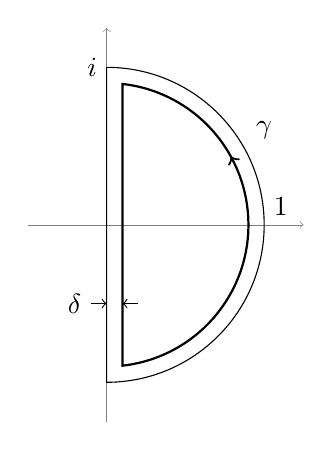
\begin{tikzpicture}[scale=2]
\def\e{0.1}
\def\r{0.9}
% axes
\draw[help lines,->](-0.5,0) -- (1.25,0);
\draw[help lines,->](0,-1.25) -- (0,1.25);
% contour
\draw [thick,decoration={markings,mark=at position 0.4 with {\arrow[thick]{>}}},postaction={decorate}]
	let \n1={asin(\e/\r)} in
	(-90+\n1:\r) arc (-90+\n1:90-\n1:\r) -- cycle;
% domain
\draw (-90:1) arc (-90:90:1) -- cycle;
% length
\draw[->] (-0.1,-0.5) -- (0,-0.5);
\draw[->] (0.1+\e,-0.5) -- (\e,-0.5);
% labels
\node[above right] at (1,0) {$1$};
\node[left] at (0,1) {$i$};
\node at (1,0.6) {$\gamma$};
\node[left] at (-0.1,-0.5) {$\delta$};
\end{tikzpicture}
\end{center}
Denote by $\tilde\Omega_\delta:=\{a\in\tilde\Omega:\min_{z_0\in\partial\tilde\Omega}|z_0-a|>\delta\}$ the interior of $\gamma$.
Define a function $\tilde g$ on $\tilde\Omega_\delta$ such that
\[\tilde g(a):=\frac1{2\pi i}\int_{\gamma}\frac{\tilde f(z)}{z-a}\,dz,\qquad a\in\tilde\Omega_\delta.\]
Note that the integrand is continuous on the contour $\gamma$, and $\tilde g$ is holomorphic on $\tilde\Omega_\delta$ by the Morera theorem, because for every affine triangle $\sigma$ in the interior of $\gamma$ we have
\[\int_{\sigma}\tilde g(a)\,dz=\int_{\sigma}\frac1{2\pi i}\int_{\gamma}\frac{\tilde f(z)}{z-a}\,dz\,da=\frac1{2\pi i}\int_{\gamma}\left[\int_{\sigma}\frac{\tilde f(z)}{z-a}\,da\right]\,dz=0\]
by the Fubini theorem and the Cauchy theorem for $\sigma$.

Moreover, for $a\in\tilde\Omega_\delta\cap\Omega$ we have 
\[\tilde g(a)=\lim_{\e\to0}\left[\frac1{2\pi i}\int_{\gamma_1}\frac{\tilde f(z)}{z-a}\,dz+\frac1{2\pi i}\int_{\gamma_1}\frac{\tilde f(z)}{z-a}\,dz\right]=\tilde f(a)+0=\tilde f(a),\]
where $\gamma_1$ and $\gamma_2$ are contours given as the folllowing figure for $\e>0$:
\begin{center}
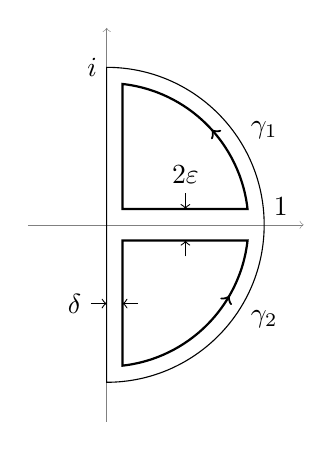
\begin{tikzpicture}[scale=2]
\def\e{0.1}
\def\r{0.9}
% axes
\draw[help lines,->] (-0.5,0) -- (1.25,0);
\draw[help lines,->] (0,-1.25) -- (0,1.25);
% contour
\draw[thick,decoration={markings,mark=at position 0.2 with {\arrow[thick]{>}}},postaction={decorate}]
	let \n1={asin(\e/\r)} in
	(\n1:\r) arc (\n1:90-\n1:\r) -- (\e,\e) -- cycle;
\draw[thick,decoration={markings,mark=at position 0.3 with {\arrow[thick]{>}}},postaction={decorate}]
	let \n1={asin(\e/\r)} in
	(-90+\n1:\r) arc (-90+\n1:-\n1:\r) -- (\e,-\e) -- cycle;
% domain
\draw (-90:1) arc (-90:90:1) -- cycle;
% length
\draw[->] (-0.1,-0.5) -- (0,-0.5);
\draw[->] (0.1+\e,-0.5) -- (\e,-0.5);
\draw[->] (0.5,0.1+\e) -- (0.5,\e);
\draw[->] (0.5,-0.1-\e) -- (0.5,-\e);
% labels
\node[above right] at (1,0) {$1$};
\node[left] at (0,1) {$i$};
\node at (1,0.6) {$\gamma_1$};
\node at (1,-0.6) {$\gamma_2$};
\node[left] at (-0.1,-0.5) {$\delta$};
\node[above] at (0.5,0.1+\e) {$2\varepsilon$};
\end{tikzpicture}
\end{center}
The same result holds also for $a\in\tilde\Omega_\delta\setminus\bar\Omega$, so we can conclude $\tilde g(a)=\tilde f(a)$ on $a\in\tilde\Omega_\delta\setminus(0,1)$, and by the contintuity of $\tilde f$ and $\tilde g$, we finally have $\tilde f=\tilde g$ so that $\tilde f$ is holomorphic on $\tilde\Omega_\delta$.
Since the above arguments make sense for every $\delta>0$ small enough, the union $\tilde\Omega=\bigcup_{\delta>0}\tilde\Omega_\delta$ implies that the function $\tilde f$ is holomorphic on $\tilde\Omega$.


(2)
The domain $\tilde\Omega$ is conformally mapped onto the upper half plane $\H=\{z\in\C:\Im z>0\}$ by
\[\f:\tilde\Omega\to\H:z\mapsto\left(\frac{z+i}{iz+1}\right)^2.\]
Note that $\f(\Omega)=\{z\in\H:|z|>1\}$.

We can compute for $(x,y)\in\tilde\Omega$
\[|\f(x+iy)|^2=\left(\frac{x^2+(y+1)^2}{x^2+(y-1)^2}\right)^2,\qquad\Im\f(x+iy)=\frac{4x(1-x^2-y^2)}{(x^2+(y-1)^2)^2}.\]
Define a function $V:\H\to\R$ such that $V:=\tilde v\circ\f^{-1}$.
Then, $V$ is a harmonic function satisfying the boundary condition
\[\lim_{(x,y)\to(x_0,0)}V(x,y)=\begin{cases}-1&\text{ if }|x_0|<1,\\1&\text{ if }|x_0|>1.\end{cases}\]
For $(x,y)\in\f(\Omega)$ so that $x^2+y^2>1$ the Poisson kernel gives that
\begin{align*}
\frac{1-V(x,y)}2
&=\frac1\pi\int_{-1}^1\frac y{(x-t)^2+y^2}\,dt\\
&=\frac1\pi\left(\tan^{-1}\frac{1-x}y+\tan^{-1}\frac{1+x}y\right)\\
&=\frac1\pi\tan^{-1}\frac{2y}{x^2+y^2-1},
\end{align*}
so
\[V(x,y)=\frac2\pi\tan^{-1}\frac{x^2+y^2-1}{2y}.\]
Thus we have for $(x,y)\in\Omega$
\[v(x,y)=V(\f(x+iy))=\frac2\pi\tan^{-1}\frac{y(1+x^2+y^2)}{x(1-x^2-y^2)}.\qedhere\]
\end{proof}

\end{document}